\documentclass[11pt]{article}
\usepackage{fancyhdr}
\pagestyle{fancy}
\newcommand\course{MATH 423}
\newcommand\hwnumber{1}
\newcommand\duedate{September 19, 2019}

\lhead{Oliver Tonnesen\\V00885732}
\chead{\textbf{\Large Assignment \hwnumber}}
\rhead{\course\\\duedate}


\usepackage{amsmath}
\usepackage{tikz}


\begin{document}


\tikzstyle{every node}=[circle,draw,fill=black,inner sep=0pt, minimum width=4pt]

\renewcommand{\thesubsection}{\thesection.\alph{subsection}}

\section{} % Section 1
($\Longrightarrow$): $G$ decomposes into claws, so there is a collection $c_1,\ldots,c_n$
of claws such that $\bigcup c_i=G$. For any $c_i$, there are three leaves and a
root. No root can be contained in any other claw, and no leaf can be the root of
any other claw, since it is adjacent to its root which, as mentioned, is
contained in exactly one claw. Thus there are no vertices in $G$ which are
both a root and a leaf in any one decomposition into claws. Thus we can
bipartition $G$ into those vertices that are a root in some claw, and those
that are a leaf in some claw.
\newline
\newline
($\Longleftarrow$): Consider one of $G$'s partite sets, $X$. Since every vertex in
$G$ has degree 3, deleting a vertex int $X$ from $G$ is like removing a claw
from $G$. Every time we remove a vertex from $X$, no edges incident to any
other vertices in $X$ are affected, so after any number of such deletions,
$deg(x)=3$ for all $x\in X$. Once the final vertex in $X$ has been deleted, we
have successfully decomposed $G$ into claws.


\section{} % Section 2
($\Longrightarrow$): Let $H$ be a subgraph of $G$. $H$ is bipartite since $G$ is,
and so the larger of its partite sets must contain at least half of its
vertices.
\newline
\newline
($\Longleftarrow$): We prove the contrapositive: if $G$ is not bipartite, then there
exists $H\subseteq G$ with no independent set containing at least of of $V(H)$.
\newline
\newline
$G$ is not bipartite, and so by the classification of bipartite graphs, contains
an odd cycle. Take $H$ to be this odd cycle, and denote it by $v_1v_2\ldots v_k v_1$.
$\{v_1,v_3,\ldots,v_{k-2}\}$ is clearly a maximal independent set, but it only
contains $\frac{k-1}{2}<\frac{k}{2}$ vertices, as desired.


\section{} % Section 3
Let $P=p_1\ldots p_k$, $Q=q_1\ldots q_k$. If $k>\frac{1}{2}|V(G)|$, then clearly
$P$ and $Q$ have a common vertex, so assume $k\le\frac{1}{2}|V(G)|$.
\newline
\newline
Assume for a contradiction that $P$ and $Q$ are disjoint. $G$ is connected, so
We know that there exists a path $R$ from $p_{\lceil\frac{k}{2}\rceil}$ to
$q_{\lceil\frac{k}{2}\rceil}$. We divide the rest of the proof into two cases:
\begin{align*}
\textrm{(1):}\qquad R\cap(P\cup Q)=\{p_{\lceil\frac{k}{2}\rceil},q_{\lceil\frac{k}{2}\rceil}\}\\
\textrm{(2):}\qquad R\cap(P\cup Q)\neq\{p_{\lceil\frac{k}{2}\rceil},q_{\lceil\frac{k}{2}\rceil}\}
\end{align*}
\newline
\newline
(1): Suppose WLOG that $p_i\in R$, where $p_i$ is contained in the path from
$p_{\lceil\frac{k}{2}\rceil}$ to $p_k$. Then we can construct the path
$p_1\ldots p_i\ldots q_{\lceil\frac{k}{2}\rceil}\ldots q_k$, where the path from $p_1$ to $p_i$
has length greater than $\frac{k}{2}$, and the path from $q_{\lceil\frac{k}{2}\rceil}$ to
$q_k$ has length at least $\frac{k}{2}$, leaving us with a path of length greater
than $k$, a contradiction to the assumption that $k$ is the length of a maximal
path.
\newline
\newline
(2): $R$ is disjoint from $P$ and $Q$ other than $p_{\lceil\frac{k}{2}\rceil}$ and
$q_{\lceil\frac{k}{2}\rceil}$, so we can simply construct the path
$p_1\ldots p_{\lceil\frac{k}{2}\rceil}\ldots q_{\lceil\frac{k}{2}\rceil}\ldots q_k$. If $k$ is odd, then
$p_1\ldots p_{\lceil\frac{k}{2}\rceil}$  and $q_{\lceil\frac{k}{2}\rceil}\ldots q_k$ both have length
$\frac{k+1}{2}$, so the total length of their combined path is at least $k+1$.
If $k$ is even, then $p_1\ldots p_{\lceil\frac{k}{2}\rceil}$ has length $\frac{k}{2}$,
and $q_{\lceil\frac{k}{2}\rceil}\ldots q_k$ has length $\frac{k}{2}+1$, so the
combined length of their paths is $k+1$. In both cases, this contradicts the
assumption that $k$ is the length of a maximal path.
\newline
\newline
This statement is no longer true if the word ``paths'' is replaced by ``cycles'':
\newline
\newline
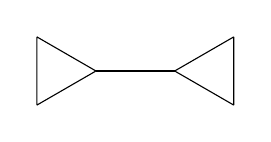
\begin{tikzpicture}
	\begin{scope}
		\draw \foreach \x in {0,120,240}
		{
			(\x:0.5) node {} -- (\x+120:0.5)
		};
	\end{scope}
	\begin{scope}[shift={(2,0)}]
	\draw \foreach \x in {60,180,300}
		{
			(\x:0.5) node {} -- (\x+120:0.5)
		};
	\end{scope}
	\draw (0.5,0) -- (1.5,0);
\end{tikzpicture}


\section{} % Section 4
Suppose for a contradiction that there exists an even graph $G$ with cut-edge
$e$. $G$ is even, and so each of its components has an Eulerian circuit. For
any of these components, if we write this circuit such that the first edge
traversed is $e$, like so: $v_1ev_2\ldots v_nv_1$, then after removing $e$,
we're left with $v_2\ldots v_nv_1$, a walk containing every vertex in that
component. Since every $u,v$-walk contains a $u,v$-path, this component remains
connected in $G-e$. In other words, $G$ and $G-e$ have the same number of
components, a contradiction to our assumption that $e$ is a cut-edge. Thus
every even graph has no cut-edge.
\newline
\newline
Given $k$, take $K_{2k+1,2k}$ and let $X$ be the larger of its partite sets.
Modify it by picking a vertex from $X$, and pairing off all the other vertices
in $X$ with an edge, like so:
\newline
\newline
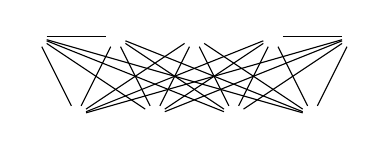
\begin{tikzpicture}
	\foreach \x in {1,2,...,5}
		\node at (\x,0) (a\x) {};
	\foreach \y in {1,2,...,4}
		\node at (0.5+\y,-1) (b\y) {};
	\foreach \x in {1,2,...,5}
	{
		\foreach \y in {1,2,...,4}
			\draw (a\x) -- (b\y);
	}
	\draw (a1) -- (a2);
	\draw (a4) -- (a5);
\end{tikzpicture}
\newline
\newline
Now every vertex except the one we chose has degree $2k+1$, so we can simply
take two copies of this graph and connect the two vertices of degree $2k$:
\newline
\newline
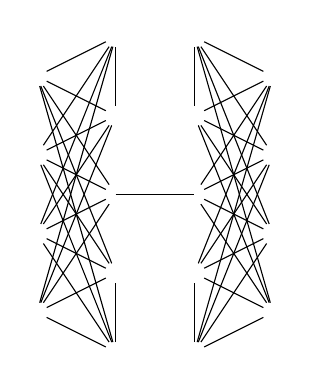
\begin{tikzpicture}
	\begin{scope}
		\foreach \x in {1,2,...,5}
			\node at (0,\x) (a\x) {};
		\foreach \y in {1,2,...,4}
			\node at (-1,0.5+\y) (b\y) {};
		\foreach \x in {1,2,...,5}
		{
			\foreach \y in {1,2,...,4}
				\draw (a\x) -- (b\y);
		}
		\draw (a1) -- (a2);
		\draw (a4) -- (a5);
	\end{scope}
	\begin{scope}[shift={(1,0)}]
		\foreach \x in {1,2,...,5}
			\node at (0,\x) (a\x) {};
		\foreach \y in {1,2,...,4}
			\node at (1,0.5+\y) (b\y) {};
		\foreach \x in {1,2,...,5}
		{
			\foreach \y in {1,2,...,4}
				\draw (a\x) -- (b\y);
		}
		\draw (a1) -- (a2);
		\draw (a4) -- (a5);
	\end{scope}
	\draw (0,3) -- (1,3);
\end{tikzpicture}
\newline
\newline
and we're left with a $(2k+1)$-regular graph with a cut edge, as desired.


\section{} % Section 5
We know that since $G\cong\overline{G}$, for every vertex in $G$ with degree
$k$, there exists a vertex in $G$ with degree $n(G)-1-k$. Define
$V_k=\{v\in V(G)\mid deg(v)=k\textrm{ or }deg(v)=n(G)-1-k\}$. The collection of
such sets forms a partition on $V(G)$. $V_k$ is guaranteed to contain an even
number of elements when $k\neq n(G)-1-k$, since each vertex of degree $k$ must
have a matching vertex of degree $n(G)-1-k$. So since there is a unique $k$ such
that $k=n(G)-1-k$, $k=\frac{n(G)-1}{2}$, and since $|V(G)|$ is odd, we have that
$V_\frac{n(G)-1}{2}$ must contain an odd number of vertices (in other wwords,
not 0). Thus there must be at least one element in $V_\frac{n(G)-1}{2}$, as desired.


\section{Bonus} % Section 6
Consider a subgraph of $D$ containing the vertices of an odd cycle in $G$ and
denote it $v_1v_2\ldots v_kv_1$. $D$ is strongly connected, so there exists a
path from $v_i$ to $v_{i+1}$ for all $i<k$, and from $v_k$ to $v_1$. We can
assume that every such path is either trivial (that is, it's just $v_iv_{i+1}$)
or that it has odd length, as if it had even length then we could simply
complete it with the edge $v_{i+1}v_i$ to obtain an odd cycle, and we would be
done. So we have a collection of $k+1$ odd paths (where $k+1$ is odd). If we
join these paths together end-to-end, we have an odd walk from $v_1$ to $v_1$.
If $v_1$ is the only repeated vertex in the walk, then it is a cycle, and we're
done. If there exists another repeated vertex, say $v$, then we can replace
$v\ldots v$ with $v$ in our $v_1v_1$ walk. We can do this until $v_1$ is the
only repeated vertex in our walk. If the resulting $v_1v_1$ walk is now even,
then one of the $vv$ paths we just removed was odd, and we're done. Otherwise,
our $v_1v_1$ path is an odd cycle, as desired.


\end{document}
